\chapter{Results}\label{sec:results}

\section{Base case}
As a reference for all following calculations, a model representing the Blennerhassett Island Bridge's final design is investigated. The results obtained by the analysis are then compared to the ones in the design drawings for plausibility. A particular challenge is the determination of the self-equilibrium stress state. As the arch was defined as an unsuitable parabola, appropriate hanger forces were determined by trial and error in the design. These permanent hanger forces of the final design are available in the drawings. However, they are unsuitable for calculating the base case, as the load distribution in the model is simplified. Instead of another trial and error procedure for the base case, the hanger forces are obtained as the result of a simultaneous arch and tie moment optimisation. Thereby, the arch's moment is weighed by a factor of 1.5 to achieve an optimal similarity. Further, the hanger forces are bounded between 25\% and 45\% of their nominal strength. The base case's internal force distributions for the permanent state are shown in Fig. \ref{fig:base_case_permanent}. Instead of the normal force in the hangers, the demand over capacity ratio is shown directly. Only the hangers of one set are shown, namely the ones inclined to the right side, and the dots are connected for readability. As a comparison, the extreme values found on the design drawings are also shown.

\begin{figure}[H]
    \centering
    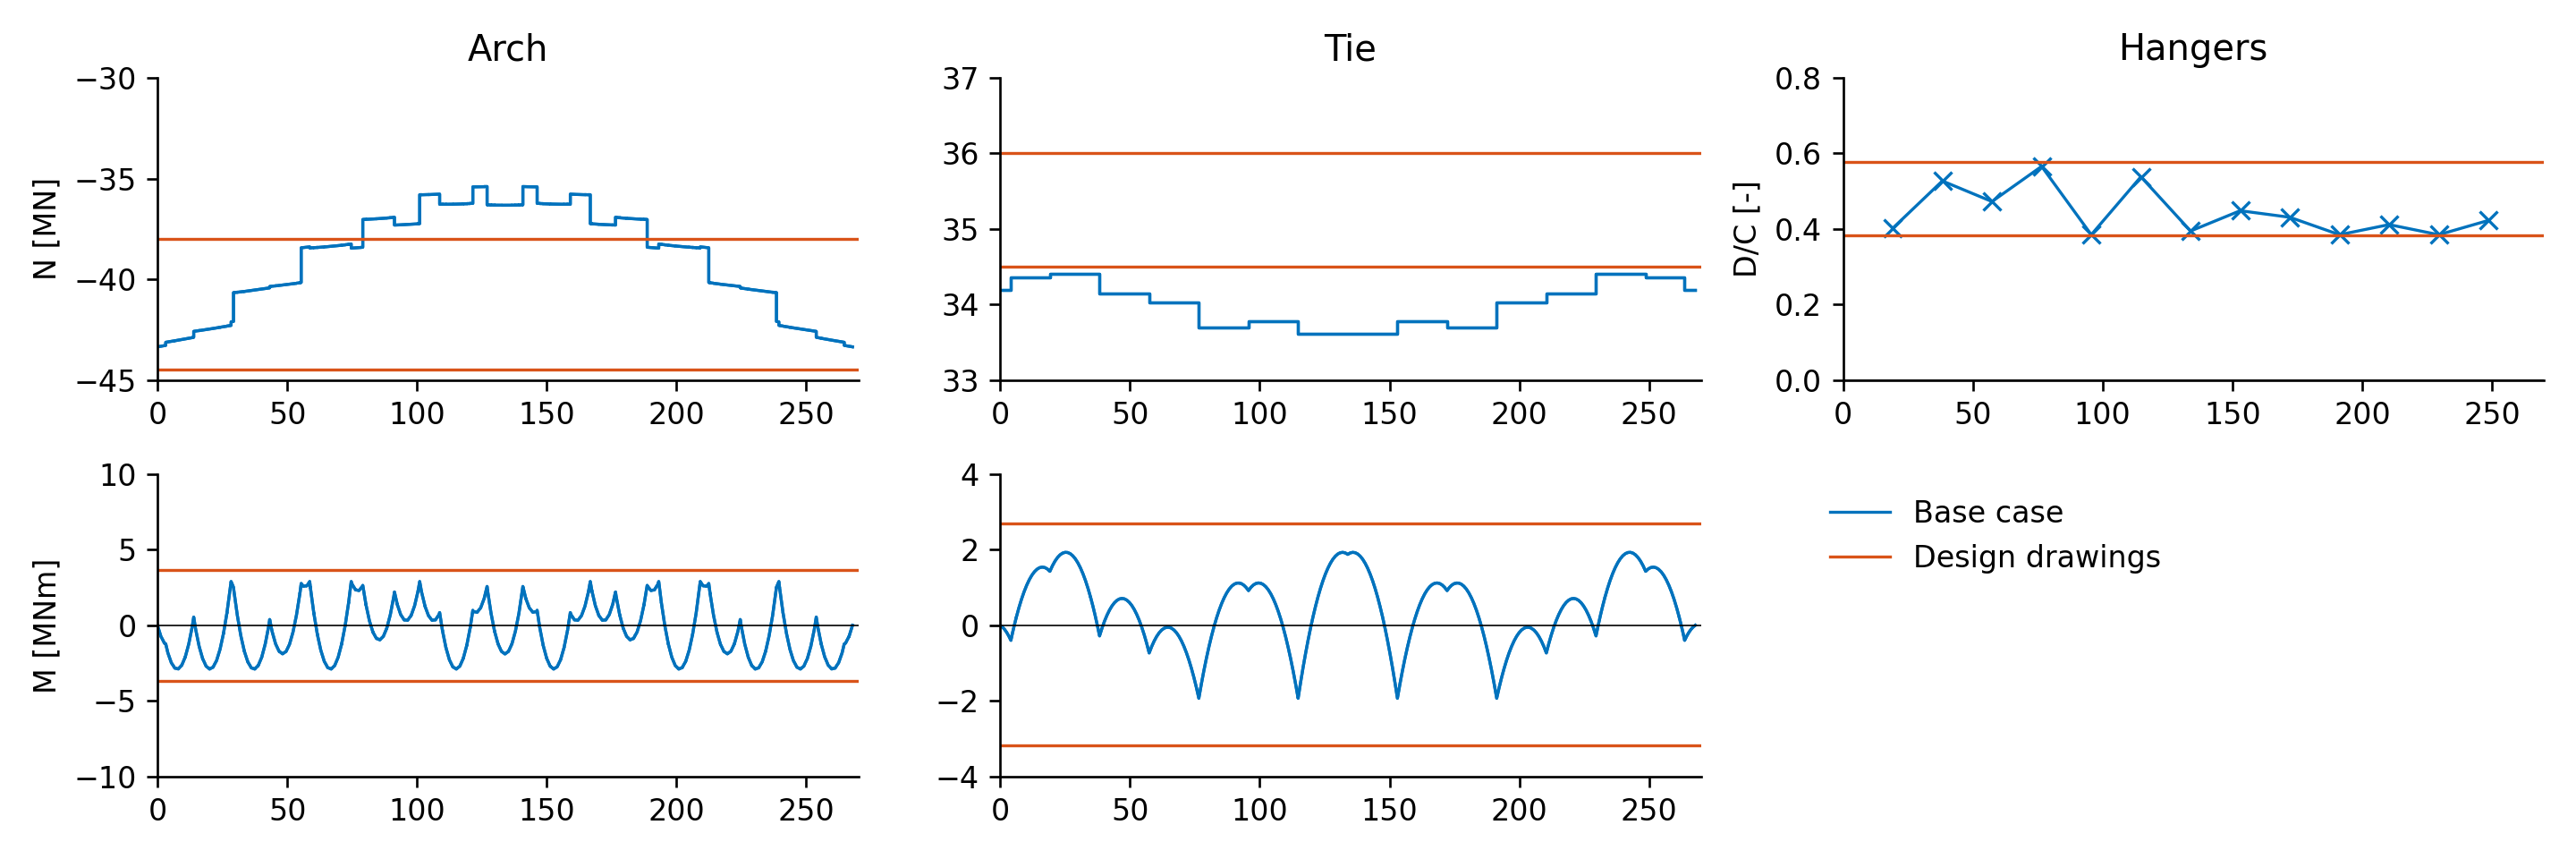
\includegraphics[width=\textwidth]{calculations/Base case/Permanent state.png}
    \caption{Permanent internal forces of the base case and reference values from the drawings}
    \label{fig:base_case_permanent}
\end{figure}

It can be seen that the moment distributions in the arch and the tie, as well as the normal forces in the hangers, match the design drawings very well. Only for the normal force in the arch rib and the tie girder an offset of \SI{2}{MN} can be observed. This difference is probably due to underestimating the weight of the bridge and its simplified assignment to the beams. However, overall the obtained internal force distribution matches the design drawings sufficiently well. It can be concluded, that for a fixed arch shape the simultaneous arch and tie moment optimisation yields adequate results.\medskip

Another comparison is drawn between the effects under characteristic live loads. As there are countless live load combinations, which are to be accounted for, it makes sense to look at the entire ranges of possible internal forces. They are shown in Fig. \ref{fig:base_case_live} by the two blue lines representing the lower and the upper limit. They are compared to the extreme values found in the design drawings.

\begin{figure}[H]
    \centering
    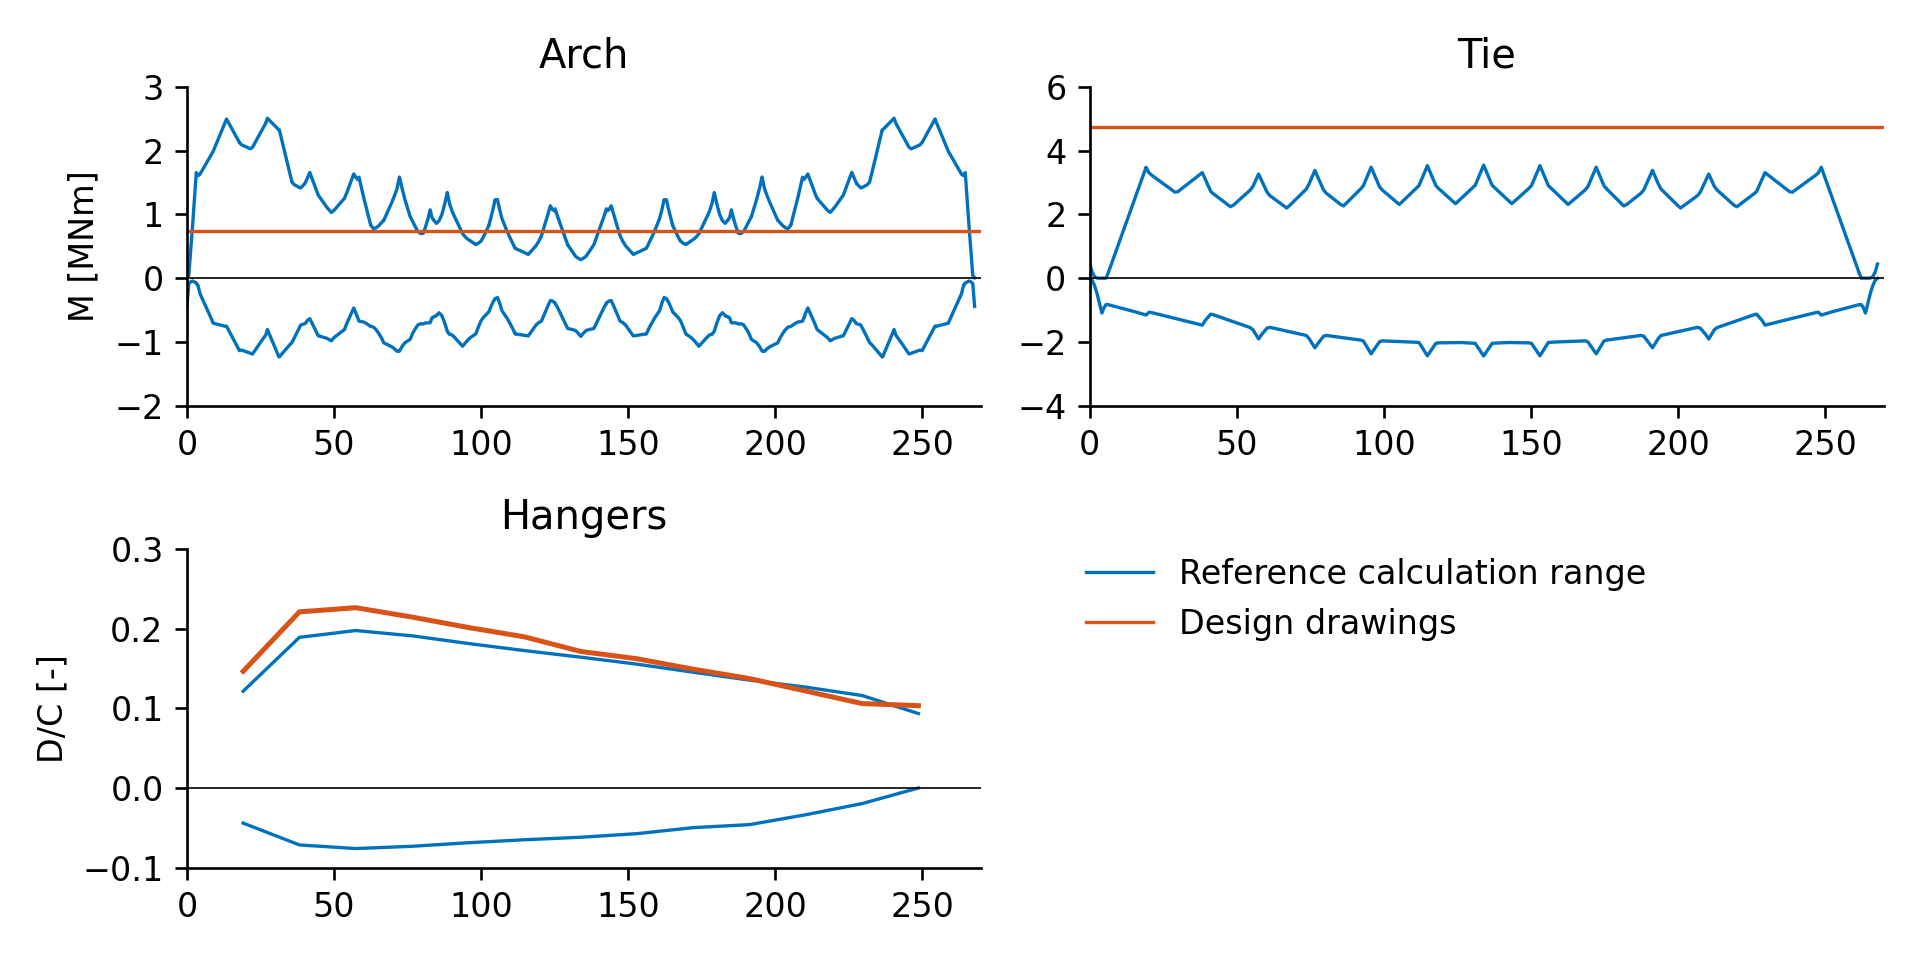
\includegraphics[width=0.8\textwidth]{calculations/Base case/Live load.png}
    \caption{Range of internal forces effects under live loading}
    \label{fig:base_case_live}
\end{figure}

The moments in the arch given in the design drawings do not correspond to the maximum for the considered load case. The considerable difference cannot be explained in another way and seems physically impossible. The moment distribution in the tie and the hangers' normal forces seem to agree on the other hand. Apparently, the live loading is only slightly overestimated in the model, which can be seen particularly well in the hangers' demand over capacity ratios. These differences are accepted, as it is not the goal of this Thesis to reproduce the results from the design drawings. Interestingly, in particular, the arch segment near the knuckle is affected by strong bending moments. On the other hand, in the tie girder, the range of effects under live loading is well distributed. Apparently, the influence lines for the moments in the tie girder at the different cross-girders follow the same shape. For the hangers, it is the second one from the knuckle connected toward the middle of the arch that undergoes the largest normal force. Towards the other side of the hanger set, the hanger forces decrease. The stronger affected hangers have in common that their inclination is closer to the arch's inclination at their respective connection node. The arch is very stiff on axial loading and comparably weaker on perpendicular forces. Therefore, at the arch nodes, smaller displacements in the hanger's direction are expected for the strongly affected hangers, explaining their higher normal forces. Only the first hanger does not follow this rule, which can be explained by its smaller area of influence. \medskip

\newpage
\section{Arch shape}
Traditionally, mainly the circle and the parabola have been used as arch shapes. The parabola has served well as a shape for traditional tied-arch bridges with vertical hangers. In this case, the vertical hanger forces on the arch are evenly distributed and the respective thrust line matches the parabola. For network tied-arch bridges, circular shapes have been considered suitable for radial arrangements. In this case, uniform hanger forces cause an approximately radial loading on the arch, which results in a circular thrust line. For a rise to span ratio of 0.2, the two shapes diverge by at most 0.8\% of the span. While this differences might seem negligible on a drawing, the impact of this difference on the arch's moment distribution is significant, as it is bigger than its usual cross-section height. In this section, the arch shape is first investigated individually as it affects the investigation of all other variables. The extreme events of cable loss are disregarded for in this investigation, because their impact is overestimated in the model. \medskip

Multiple approaches to determine the arch shape have been introduced in Section \ref{sec:met_arch}. All of them are linked to the thrust line, which is approximately the most efficient shape. The following four arch shapes are compared in this investigation.
\begin{enumerate}
    \item Thrust line: This shape is obtained numerically as the thrust line for the hanger forces obtained from a tie moment optimisation. The respective hanger forces are uniform at $N_p=\SI{2.4}{MN}$ which corresponds to 45\% of their characteristic resistance.
    \item Polynomial thrust line approximation: The above thrust line is approximated by a quartic function. The quartic function is described by Eq. \eqref{eq:polynomial_shape} and the shape parameter $b$. This parameter is obtained by a least squares approximation. It fulfills the conditions $y(0)=r$ and $y(s/2)=0$
    \begin{equation}
        y(x)=r \cdot \left(1 - b \cdot \left(\frac{2\,x}{s}\right)^2 - (1-b) \left(\frac{2\,x}{s}\right)^4 \right)
        \label{eq:polynomial_shape}
    \end{equation}
    \item Spline thrust line approximation: As a second approximation of the thrust line a cubic spline defined by the arch-hanger connection nodes is used. These nodes are therefore represented at their exact location.
    \item Thrust line of continuous hanger arrangement: This shape is the thrust line of the hypothetical continuous hanger arrangement, which was introduced in Section [].
\end{enumerate}

These shapes are hardly distinguishable by eye. To make their differences visible, only their respective deviations to the parabolic shape are shown in Fig. \ref{fig:arch_shapes_13}. Also a circular arch is shown to put the results into perspective.

\begin{figure}[H]
    \centering
    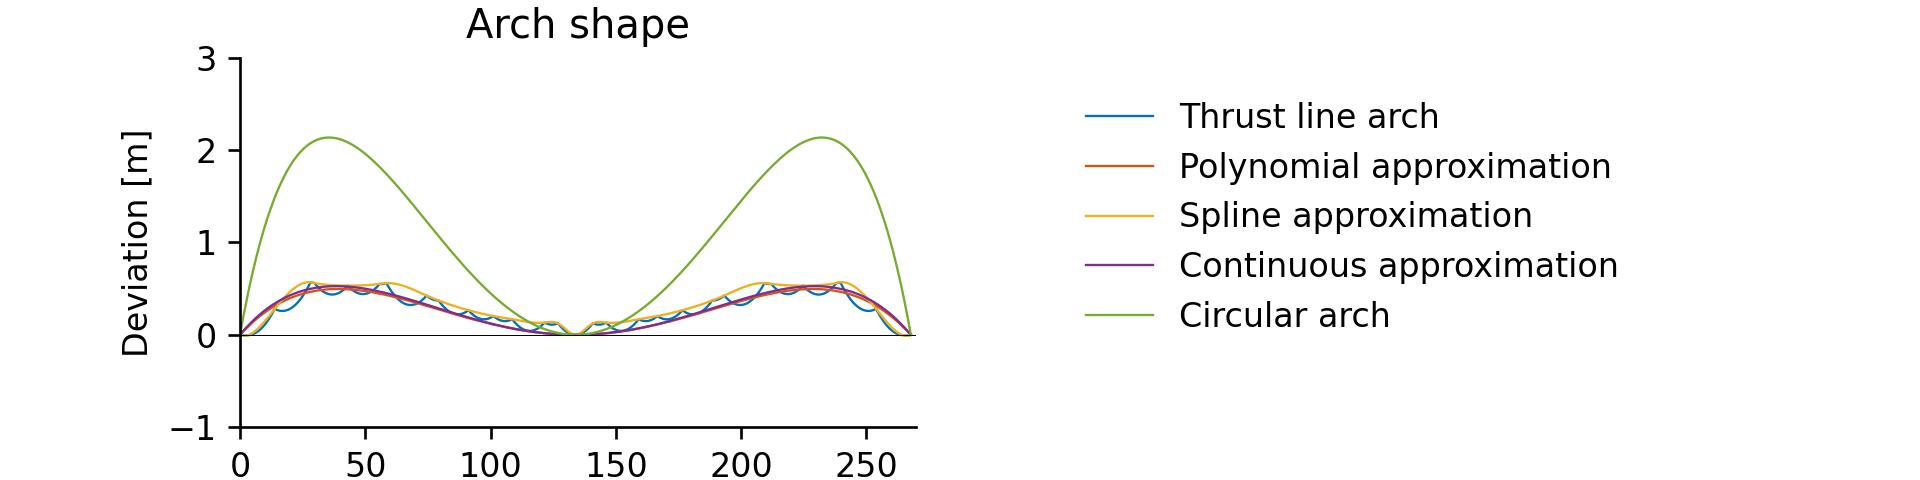
\includegraphics[trim={0 0 2cm 0},clip, width=0.8\textwidth]{calculations/arch shape/arch_shapes_13.png}
    \caption{Deviation of arch shapes from parabolic shape}
    \label{fig:arch_shapes_13}
\end{figure}

In the range between the circular and the parabolic shape, the thrust line tends slightly to the parabolic side. From the similarity between the polynomial and the continuous approximation, it can be concluded, that if the hanger arrangement is dense enough, a quartic function can yield an appropriate arch shape for this hanger arrangement pattern. All three approximations seem to fit the thrust line reasonably well. But to investigate the impacts of the remain deviations from the thrust line, the corresponding permanent moment distribution is presented in Fig. \ref{fig:arch_permanent_moments_13}.

\begin{figure}[H]
    \centering
    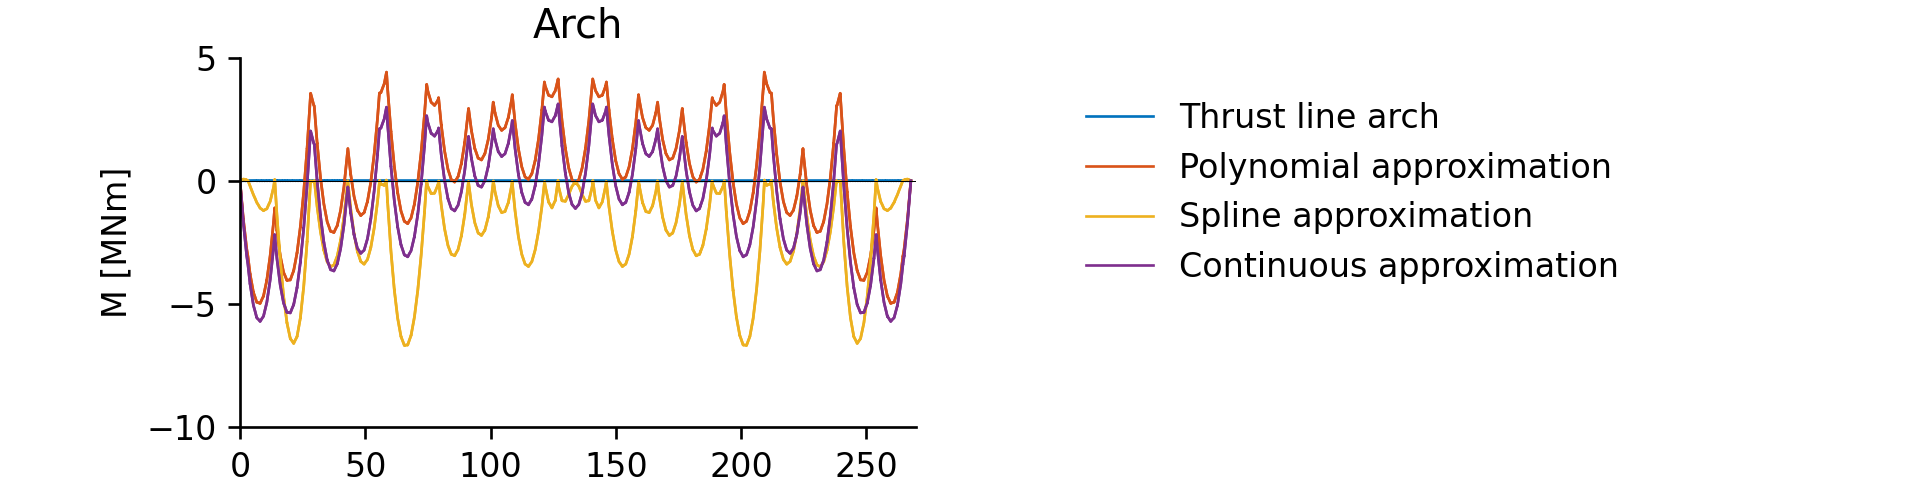
\includegraphics[trim={0 0 2cm 0},clip, width=0.8\textwidth]{calculations/arch shape/permanent state_13.png}
    \caption{Permanent arch moment distributions depending on arch shape}
    \label{fig:arch_permanent_moments_13}
\end{figure}

Despite the apparent match of the arch shapes, significant bending moments result in each of the three approximations. The spline approximation's moment distribution is strictly negative, which relies on the characteristic that a spline lies above the approximately linear thrust line and only matches it at the connection nodes. It is particularly interesting, that all approximations feature a similar parabolic moment distribution between the arch-hanger connection nodes. While these moment distributions resulting for the approximated shapes are certainly considerable, it is practically infeasible to find a simple shape matching the arch thrust line. Any shape with an approximately constant radius $R$ results in a certain deviation from the thrust line and the corresponding moment deviation $\Delta M$. This deviation can be approximated depending on the distance between two hanger points $d$ and the arch's normal force $N$ according to Eq. \eqref{eq:moment_deviation}.

\begin{equation}
    \Delta M=-\left(R-\sqrt{R^2-\left(d/2\right)^2}\right) \cdot N
    \label{eq:moment_deviation}
\end{equation}

For the Blennerhassett Island Bridge, these variables roughly correspond to $R=\SI{194}{m}$, $d=\SI{17}{m}$ and $N=\SI{40}{MN}$. Eq. \eqref{eq:moment_deviation} yields a moment deviation of $\Delta M=\SI{7.5}{MNm}$ coming close to the value observed in Fig. \ref{fig:arch_shapes_13}. From the analytical form of Eq. \eqref{eq:moment_deviation} it can further be concluded, that a reduction of the hanger node spacing has a more than proportional impact on the bending moment deviation. To put these deviations into the context of the design verifications, the demand over capacity ratios resulting in the arch are shown in Table \ref{tab:arch_shape_dc_13}.

\begin{table}[H]
    \centering
    \input{calculations/arch shape/dc_comparison_13.txt}
    \caption{Arch design verifications (neglecting extreme events)}
    \label{tab:arch_shape_dc_13}
\end{table}

The deviations from the thrust line of the considered arch shapes increase the demand over capacity ratios by 0.05 on average. This difference is not critical for the initial design, but it offers some potential for optimisation. Further, it should be noted that also the exact thrust line is not the most efficient arch shape. In the strength limit state for vehicular use, the arch is affected by stronger positive bending moments than negative ones, as shown in Fig. \ref{fig:arch_shape_strength_1}. Therefore, a certain positive deviation from the thrust line and the resulting negative bending moment can prove beneficial to the verifications. This potential was estimated by evaluating the difference of the maximum and minimum bending moments in the decisive limit state and comparing it to the resistance. The comparison yielded possible reductions for the three segments between 0.01 and 0.03.

\begin{figure}[H]
    \centering
    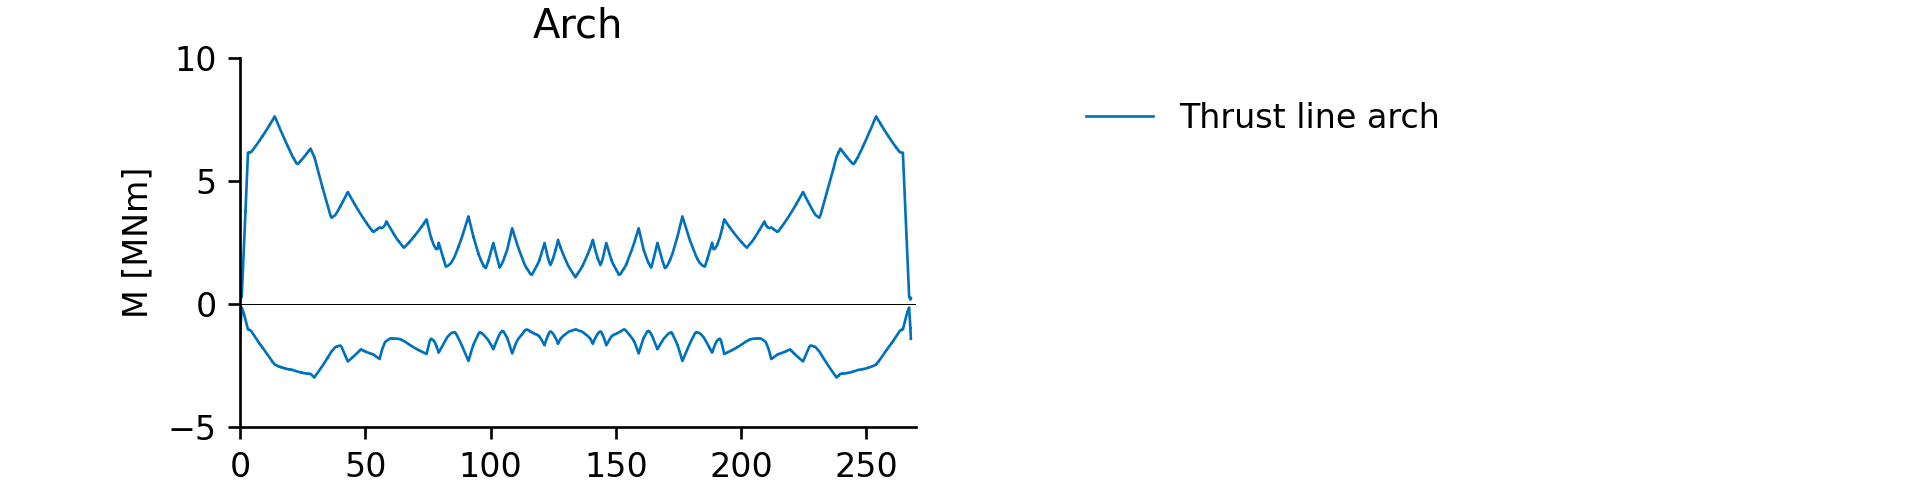
\includegraphics[trim={0 0 2cm 0},clip, width=0.8\textwidth]{calculations/arch shape/strength-I_13.png}
    \caption{Range of moments in the strength-I limit state}
    \label{fig:arch_shape_strength_1}
\end{figure}

Ultimately, the influence of the hanger density on the arch shape is investigated. It was concluded from Eq. \eqref{eq:moment_deviation}, that by reducing the distances between the hangers an over-proportional reduction in the permanent moment distribution results. Therefore, a similar calculation of the four arch shapes with 26 hangers per set was conducted. The resulting arch shapes are presented in Fig. \ref{fig:arch_shapes_26}.

\begin{figure}[H]
    \centering
    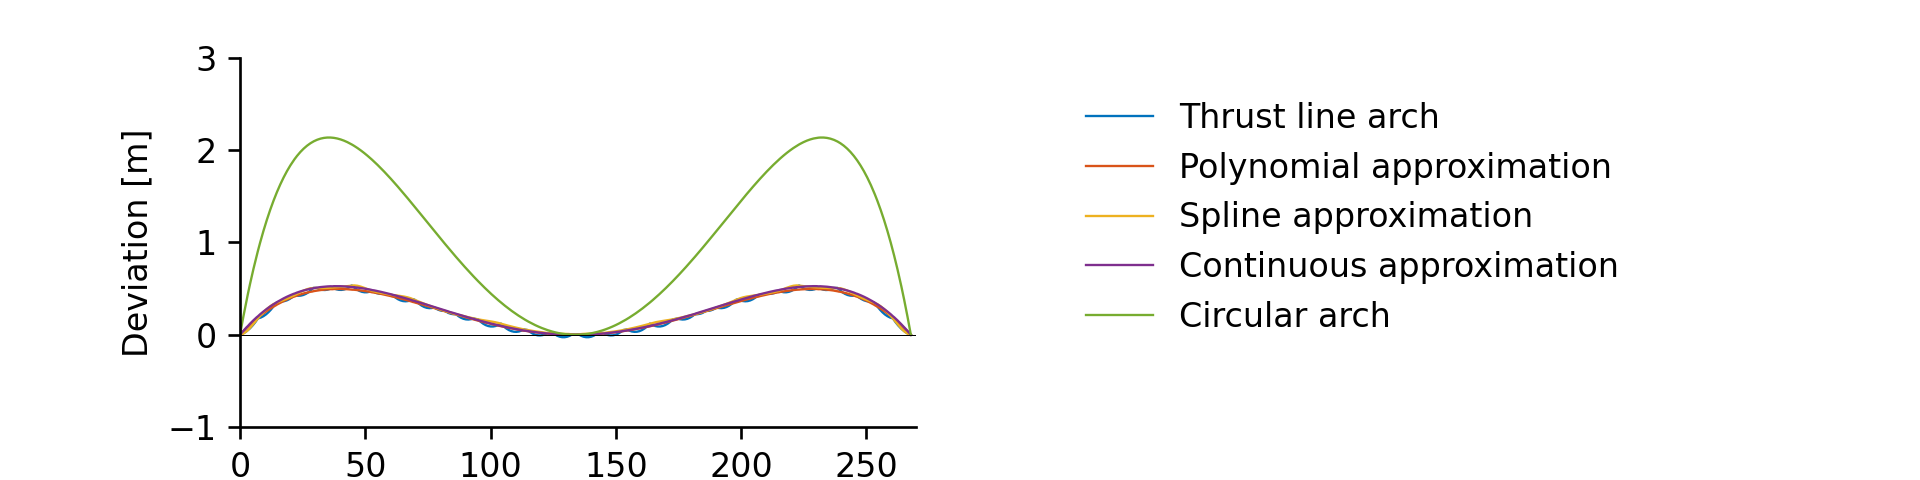
\includegraphics[trim={0 0 2cm 0},clip, width=0.8\textwidth]{calculations/arch shape/arch_shapes_26.png}
    \caption{Deviation of arch shapes from parabolic shape (26 hangers)}
    \label{fig:arch_shapes_26}
\end{figure}

If the amount of hangers is large enough, all considered approximations yield suitable arch shapes. The impact of the remaining deviation from the thrust line on the design verifications is negligible, as can be seen in the uniform demand over capacity ratios presented in Table \ref{tab:arch_shape_dc_26}. For the initial design, especially the continuous approximation presents a promising arch shape, as it does not involve a specific thrust line calculation. However, for sparse hanger arrangements, a more accurate modelling of the thrust line, involving the characteristic kinks, might be inevitable for the arch shape.

\begin{table}[H]
    \centering
    \input{calculations/arch shape/dc_comparison_26.txt}
    \caption{Arch design verifications (26 hangers, neglecting extreme events)}
    \label{tab:arch_shape_dc_26}
\end{table}


\newpage
\section{Hanger density}
A denser hanger arrangement provides multiple benefits. As seen in the previous chapter, the shape deviation moments are reduced through the corresponding reduction of the distances between the hangers' anchorages. Further, the effects in the extreme event of cable loss are significantly lowered, as the hanger forces are reduced inverse proportionally to the increase of hangers. Also the impaired structural system loses less of its essential stiffness and undergoes additionally lower effects therefore. However, the challenging task is to find an appropriate self-equilibrium stress state for structural systems in which the locations of the floor beams and the hangers do not coincide on the tie girder. \medskip

In this investigation, this challenge is tackled by tie moment optimisation method. It allows finding the permanent hanger forces within a certain range minimising the resulting moment distribution in the tie girder. This range is set between 25\% and 40\% of the hangers' characteristic capacity.  Four bridges are analysed featuring 13, 20, 26 or 27 hangers per set and a constant amount of 13 floor beams. The arch shapes are defined as the quartic polynomial approximation of the thrust line. The model featuring 26 hangers is shown in Fig. \ref{fig:structure_26}. The spacing between the knuckle and the first hanger is slightly increased so there is an equally spaced pair of hangers around every floor beam. While the arrangement appears dense, the hanger spacing on the tie girder is still around \SI{10}{m} representing a rather high value for modern network tied-arch bridges.

\begin{figure}[H]
    \centering
    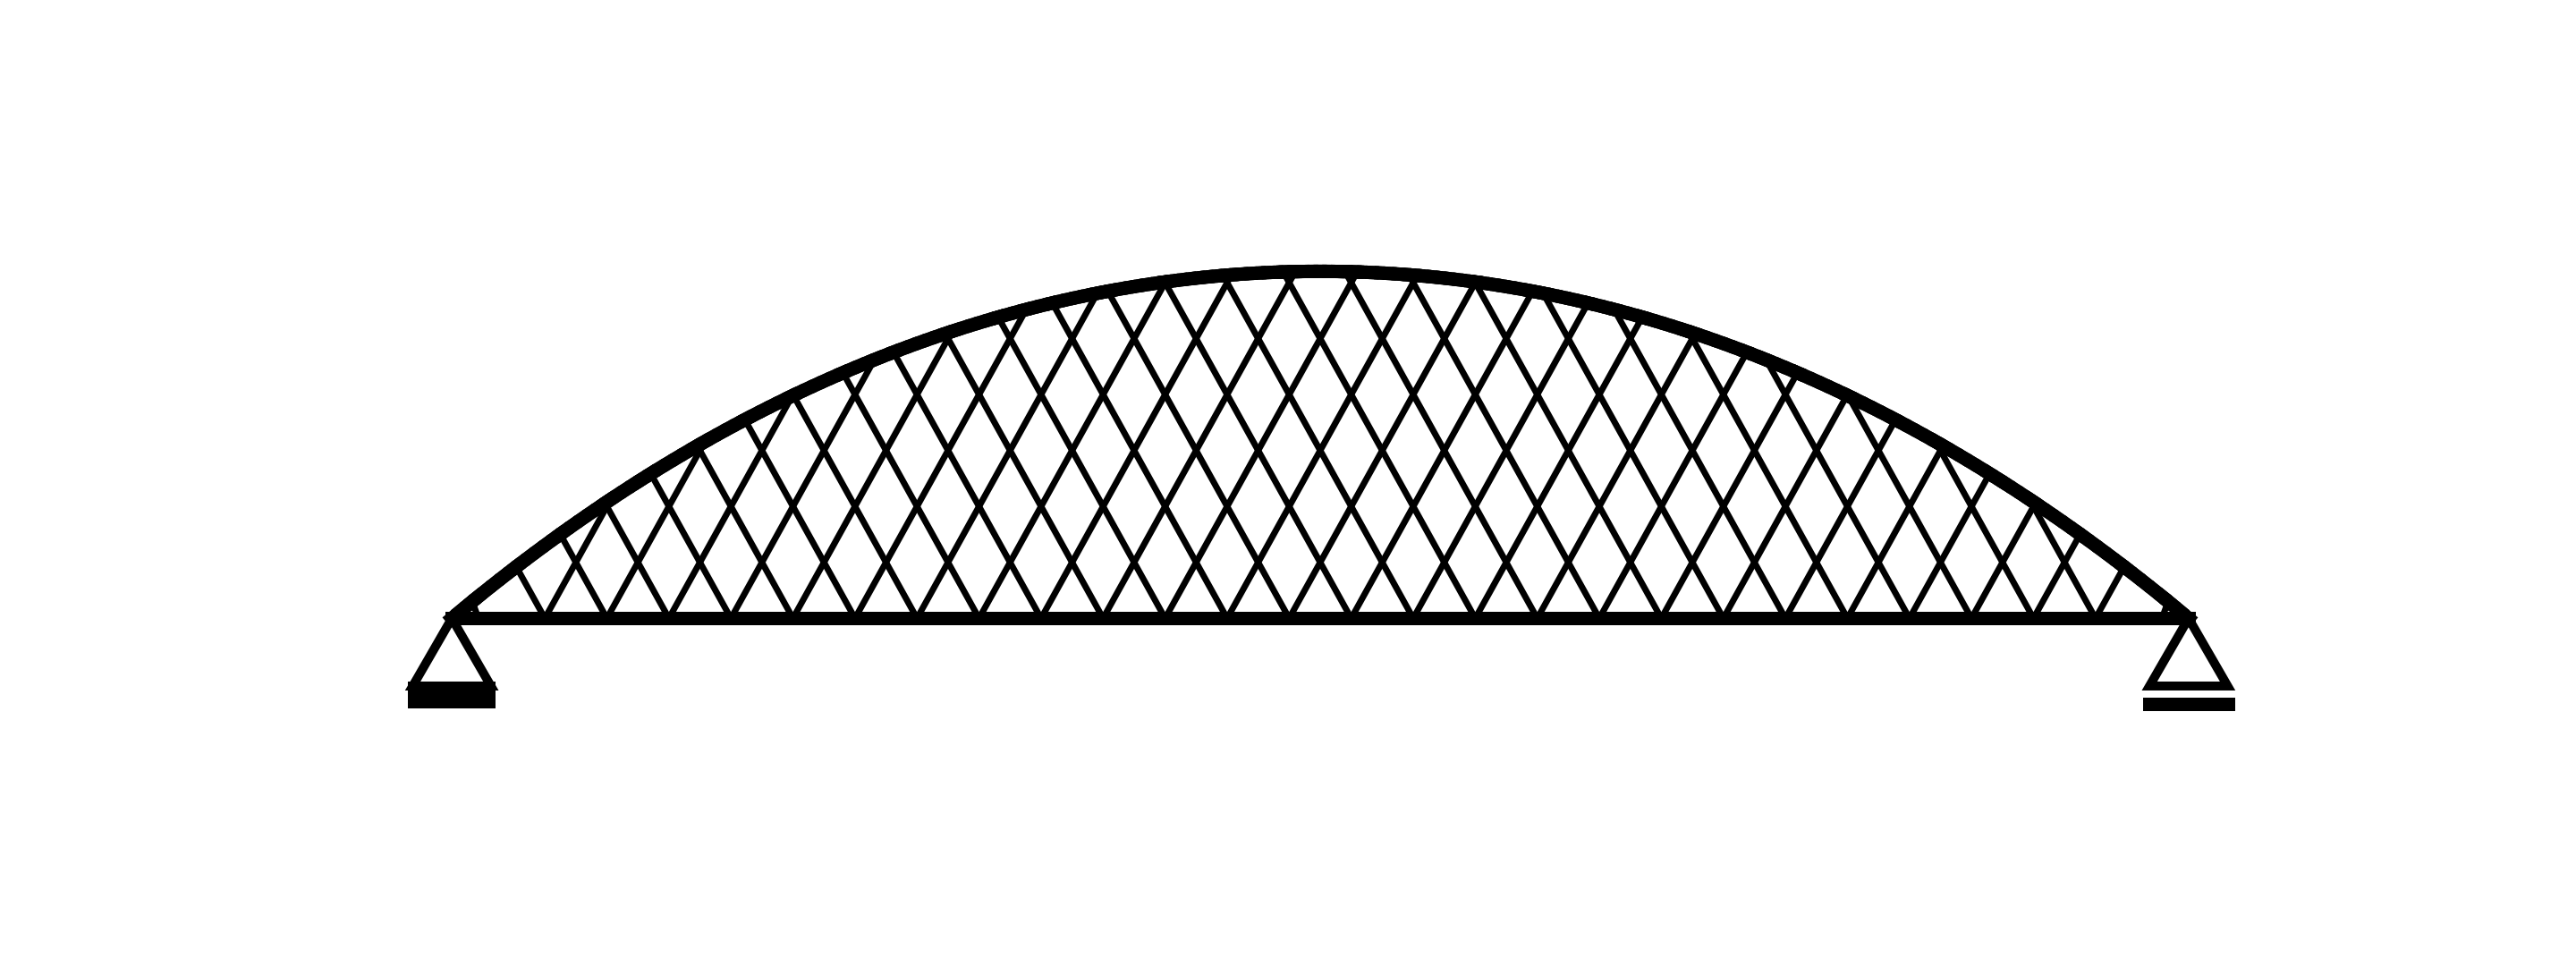
\includegraphics[trim={0 1cm 0 1cm},clip, width=0.7\textwidth]{calculations/hanger amount comparison/structure_26.png}
    \caption{Structural model of a dense hanger arrangement (26 hangers per set)}
    \label{fig:structure_26}
\end{figure}

The optimised effects under permanent loads are shown in Fig \ref{fig:hd_permanent}. As expected from the investigation of the arch shape, the bending moments in the arch are lowered for an increased hanger density. However, in the knuckle region of the arch the strong bending moments are retained for the arrangements with 20 and 27 hangers per set. They are due to the tie moment optimisation method assigning significant supernumerary moments to the knuckle. The quartic polynomial approximation is not able to match the corresponding thrust line.

\begin{figure}[H]
    \centering
    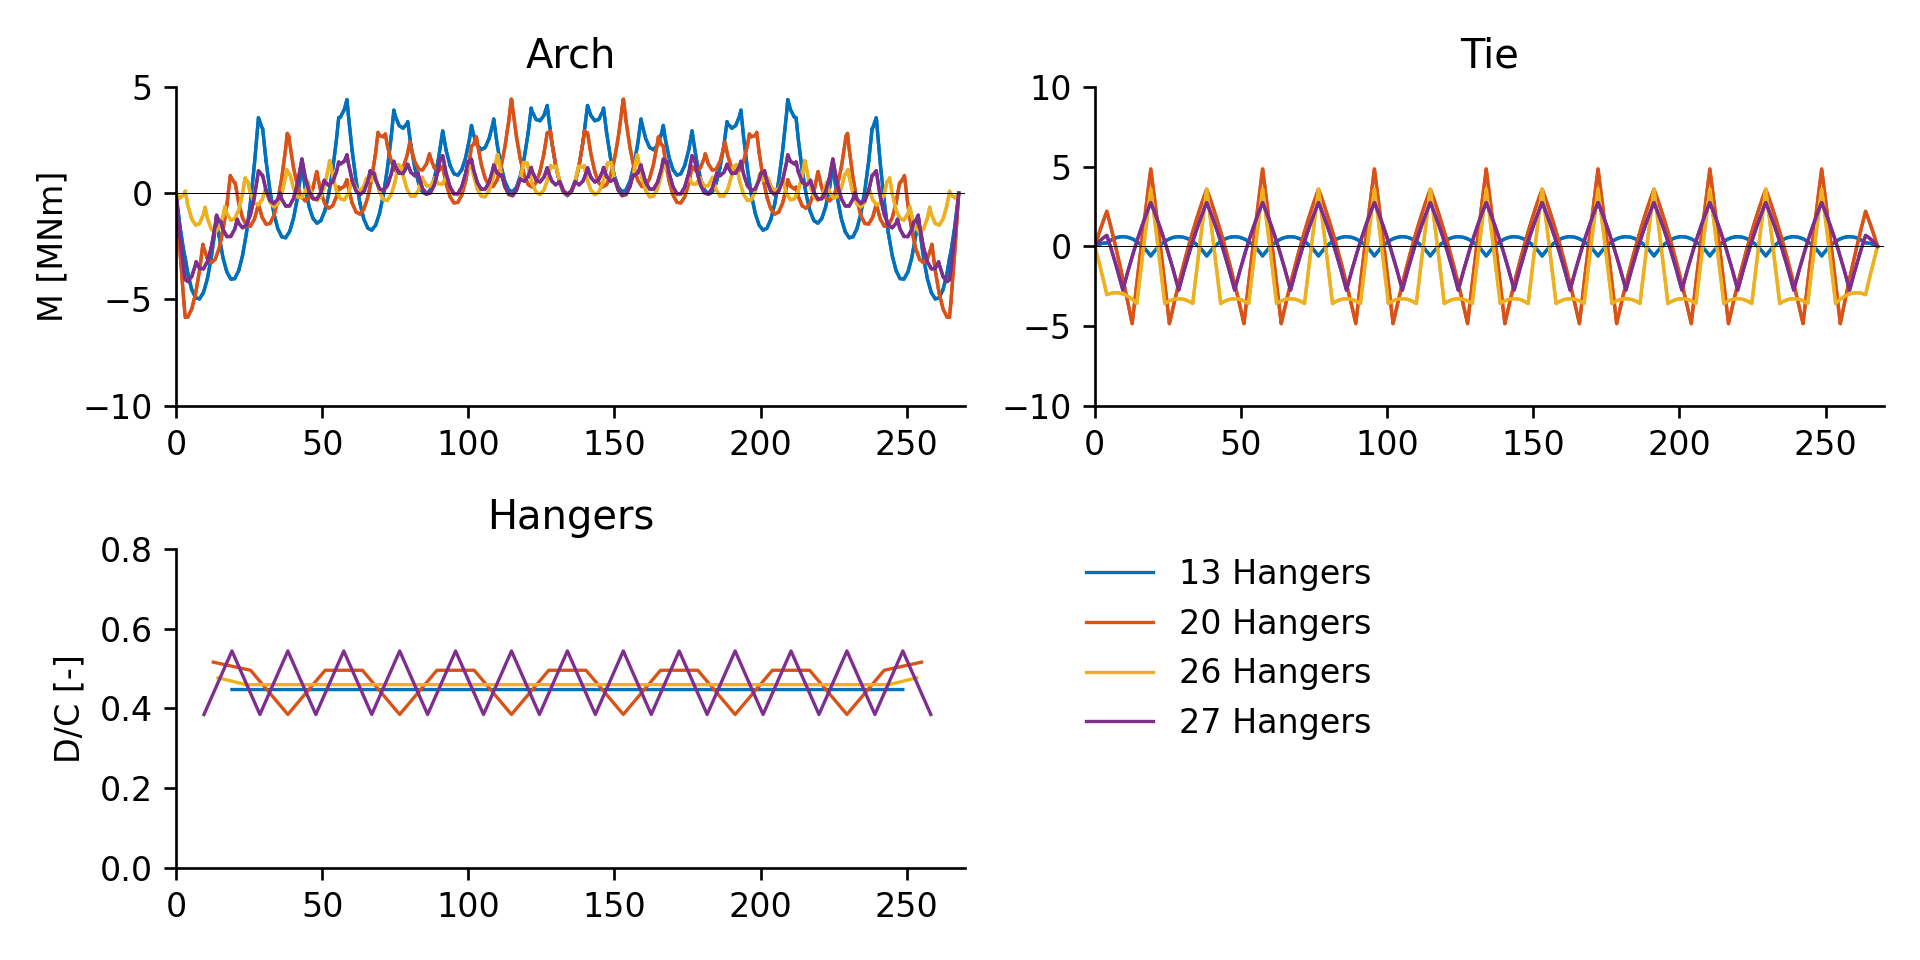
\includegraphics[width=0.9\textwidth]{calculations/hanger amount comparison/permanent state.png}
    \caption{Optimised permanent effects for different hanger densities}
    \label{fig:hd_permanent}
\end{figure}

The permanent hanger forces are no longer constant for the models with 20 and 27 hangers, as the hangers near the floor beams carry the majority of the forces. At the same time a strong bending moment distribution in the tie is inevitable. The model featuring 26 hangers seems slightly more suitable as it is able to retain constant hanger forces and also a slightly lower tie moment distribution. Further, the elastic responses to dead loading are shown in Fig. \ref{fig:hd_elastic_response_dl}.
%On top of the disadvantageous permanent effects, also the elastic response of the modified models to live loading, which are shown in Fig. \ref{fig:hd_live}, seem unfavourable.

\begin{figure}[H]
    \centering
    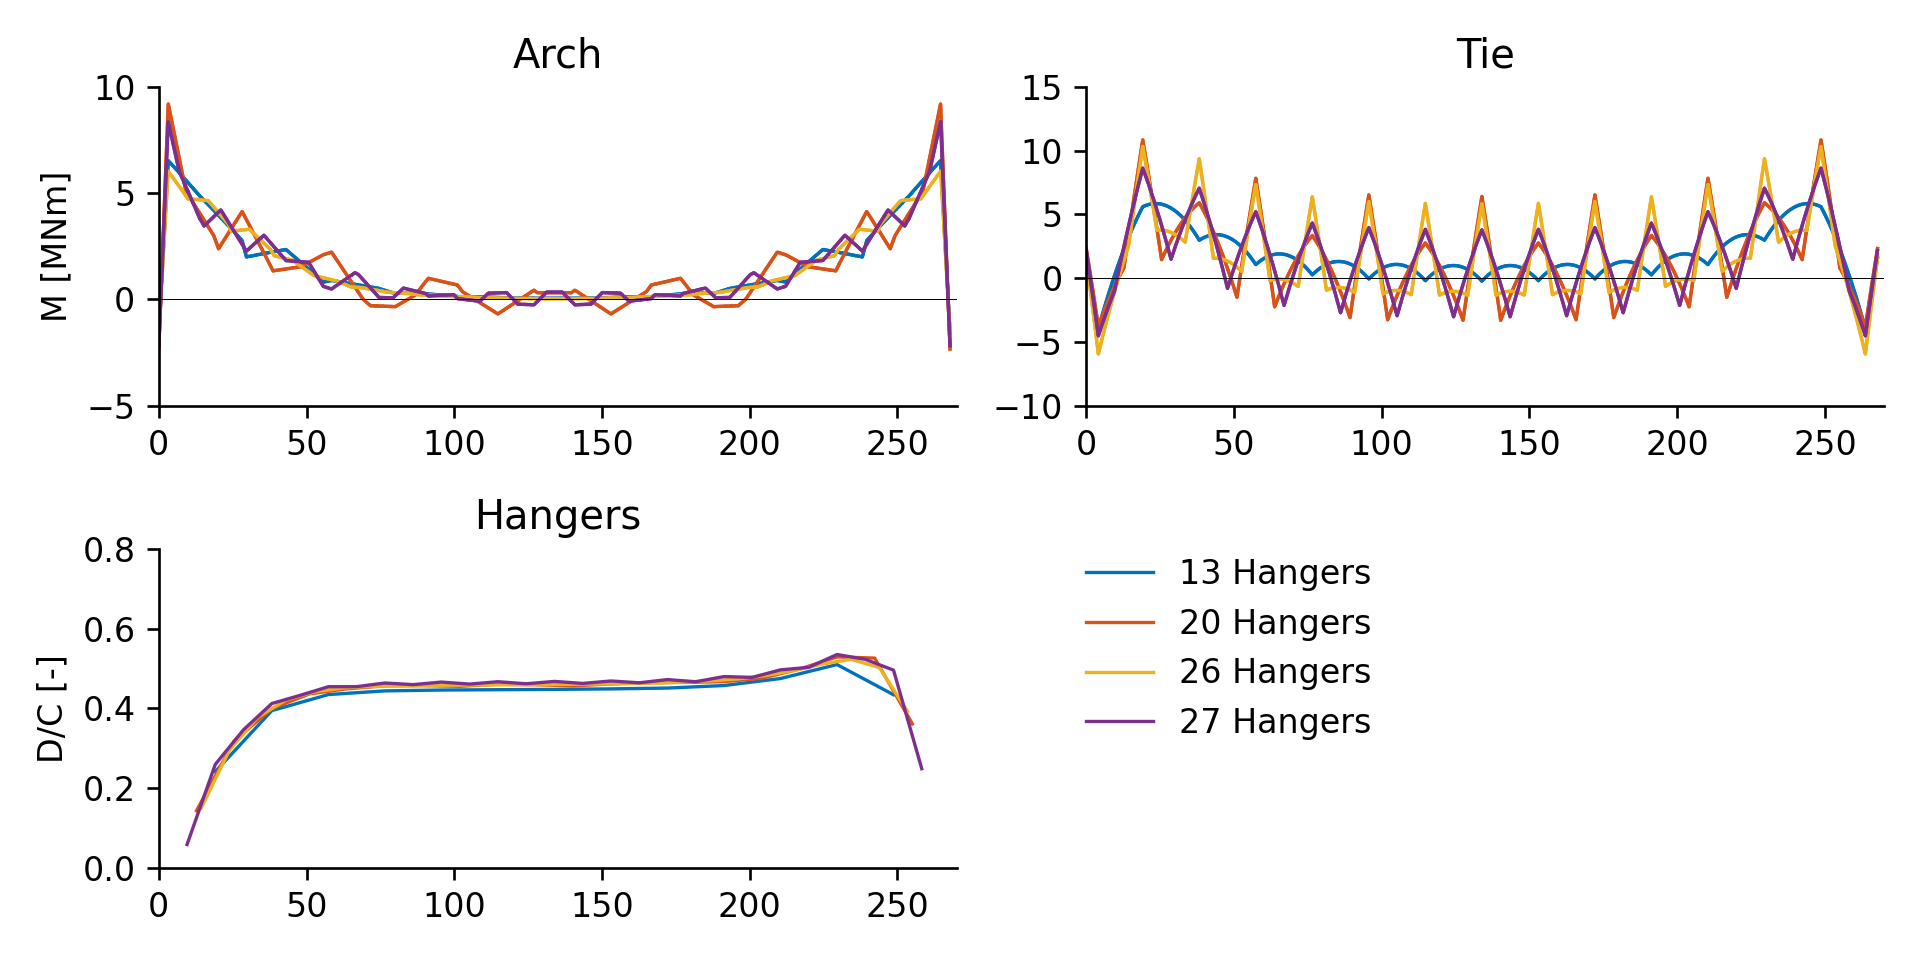
\includegraphics[width=0.8\textwidth]{calculations/hanger amount comparison/dead load.png}
    \caption{Elastic response to dead loading for different hanger densities}
    \label{fig:hd_elastic_response_dl}
\end{figure}

While these effects are already included in the permanent effects, they are still relevant for the design verifications as they are increased or decreased therefor. While the response of the arch and the hangers remains approximately identical, the tie is again affected by stronger bending moments in the denser models. This characteristic is accentuated by the range of tie moments relevant for the tie fracture extreme event, presented in Fig. \ref{fig:hd_tie_fracture}.

\begin{figure}[H]
    \centering
    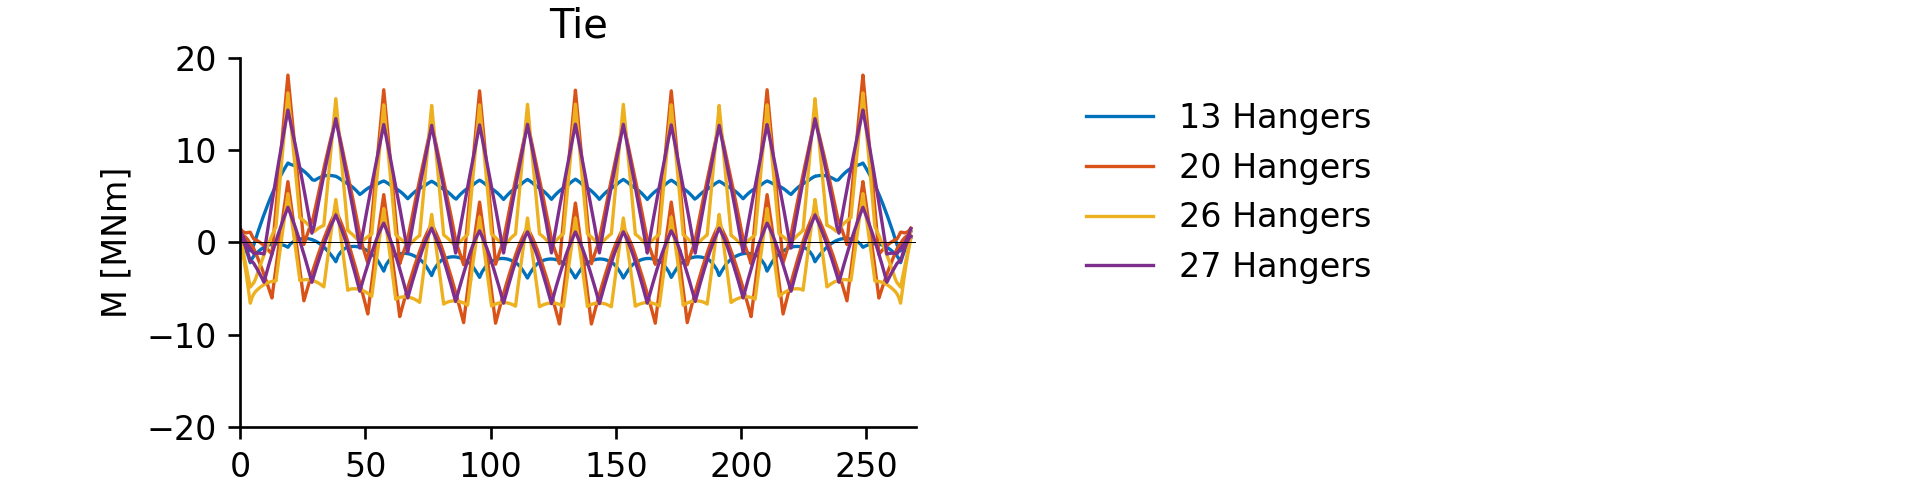
\includegraphics[trim={0 0 3cm 0},clip, width=0.8\textwidth]{calculations/hanger amount comparison/tie fracture.png}
    \caption{Range of tie bending moment for tie fracture extreme event}
    \label{fig:hd_tie_fracture}
\end{figure}

The previously rather uniform moments became particularly peaky. The corresponding design verification in the tie is thereby significantly impaired, as show in Table \ref{tab:hd_dc}. An optimisation of the hanger density itself, therefore renders no potential for optimisation, even though the cable loss extreme event improves as expected.

\begin{table}[H]
    \centering
    \resizebox{\columnwidth}{!}{%
    \input{calculations/hanger amount comparison/dc_comparison.txt}
    }
    \caption{Design verifications for different hanger densities}
    \label{tab:hd_dc}
\end{table}


\section{Floor beam density}
It was seen in the previous chapter, that it is impossible to obtain an optimised design with more hangers per set than floor beams. To facilitate the design verifications in the extreme event of cable loss, a denser hanger arrangement has to be paired with a higher floor beam density. It seems a particularly reasonable step, as the Blennerhassett Island Bridge holds the record for hanger spacing on the tie girder at \SI{20}{m}. This was only feasible as the extreme event of floor beam loss was not considered in the design. However, there are other causes to investigate the floor beam and hanger density. Besides the previously mentioned improved behaviour under cable loss and smaller deviations of the arch from the thrust line, a general more continuous transfer of loads might be beneficial. \medskip

Theoretically, an adapted floor beam spacing changes the entire deck system and its weight. However, the deck is not subject to this investigation and it is therefore assumed, that the total weight of the deck system and the floor beams is constant and independent of the floor beam spacing. Four models with different floor beam and hanger densities are investigated in this Section. Besides the final design with 13 floor beams, models with 10, 20 and 27 floor beams are investigated. As an advantage for the sparse model with 10 floor beams, the actual thrust line is assumed as the arch shape. For the other models, the thrust line is approximated by the quartic polynomial. The respective permanent effects are shown in Fig. \ref{fig:fb_permanent}.

\begin{figure}[H]
    \centering
    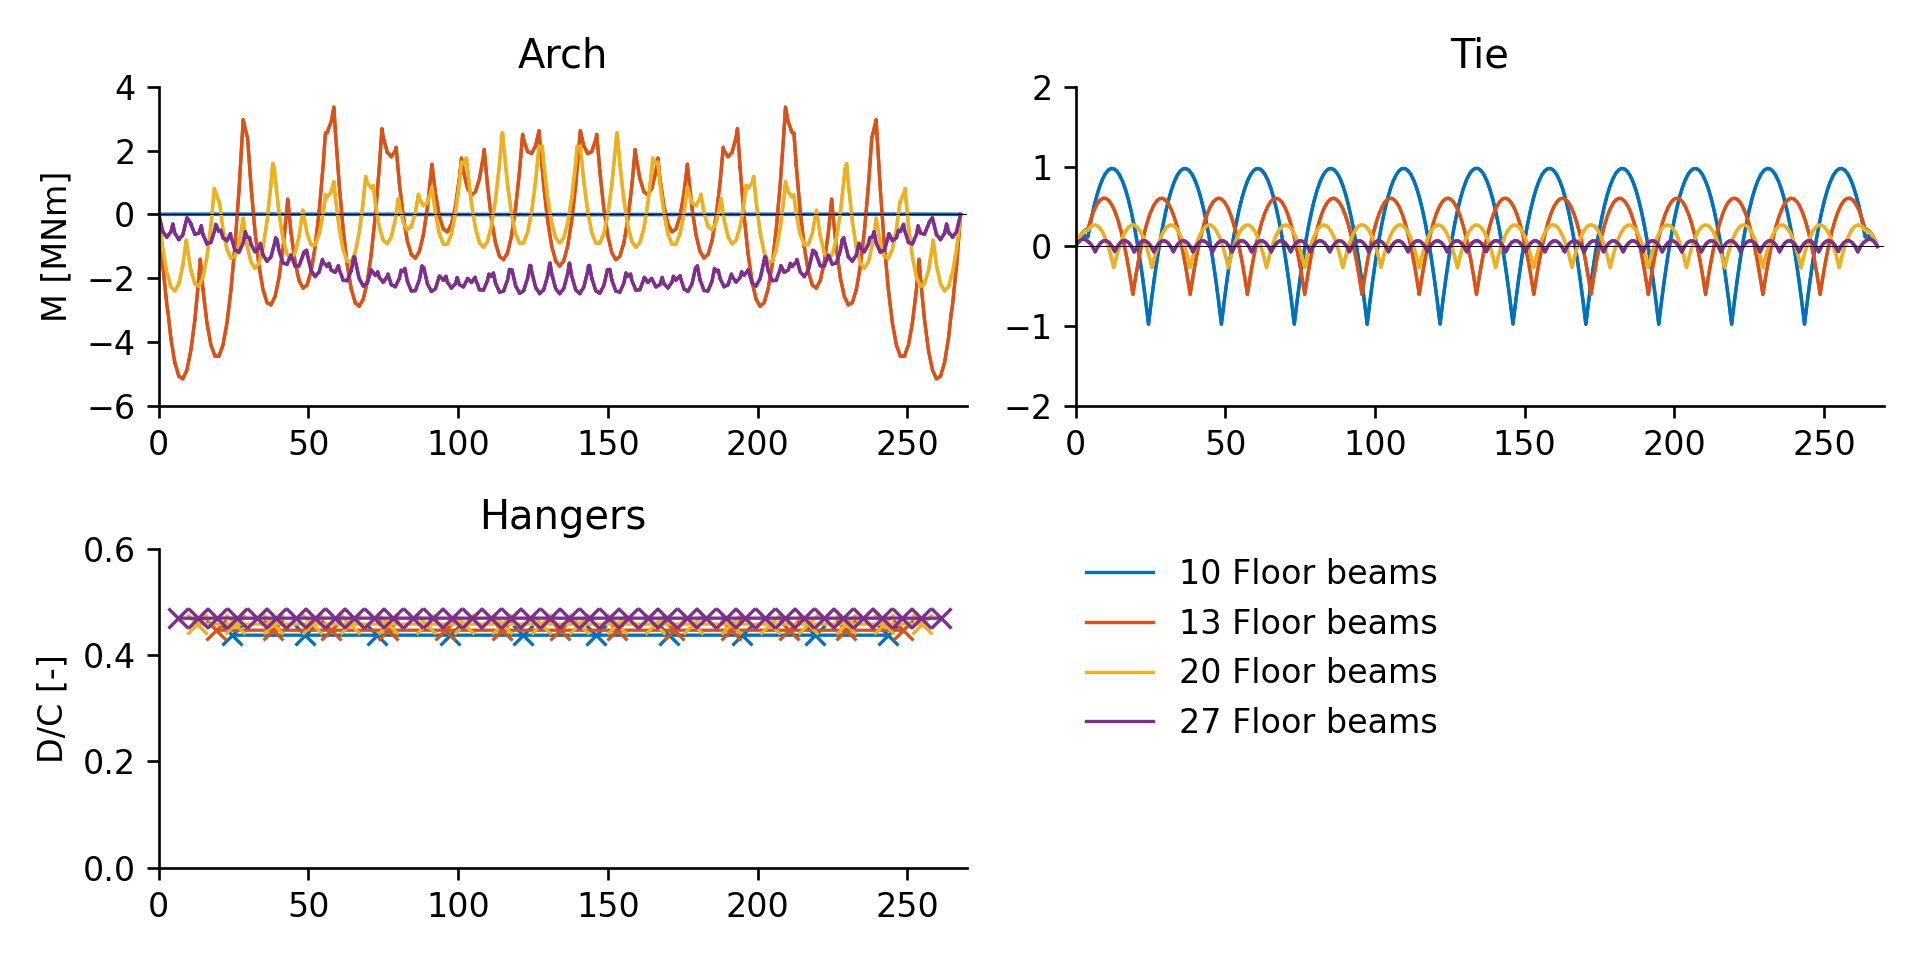
\includegraphics[width=0.8\textwidth]{calculations/floor beam comparison/permanent state.png}
    \caption{Optimised permanent effects for different floor beam densities}
    \label{fig:fb_permanent}
\end{figure}

All models retain the characteristic permanent effects resulting from the tie optimisation, which are the uniform hanger forces and a uniform tie moment distribution with peaks at $M=\pm\,g_{Tie} \cdot s^2 / 16$. It can be seen, that the hanger forces slightly increase, as less weight of the deck is directly carried by the floor beam at the knuckle. Compared to the other models, the permanent arch moments for 13 floor beams seem to be significant. However, it is known from the investigation of the arch shape, that the moments only lower the demand over capacity ratio by about 0.05. \medskip

In Fig. \ref{fig:fb_live} the elastic response under characteristic live loading is shown. For the hangers, the response is practically unchanged. Only the hangers very close to the knuckle undergo a lower normal force, as the tie girder at the knuckle carries the corresponding load directly to the knuckle. For the tie girder, the moment effects increase with the floor beam density and constitutes a slightly impairing impact on the design verifications. The stronger moments are due to the weaker coupling of the tie and the arch at the floor beams. While the force at the floor beams for the distributed lane load decreases, the force of the design trucks remain the same. They are responsible for the slightly increased hanger forces and bending moments in the tie girder. The moment distribution on the arch rib shows a different tendency. Overall the effects of the models resemble a similar shape. However, for fewer floor beams, certain moment peaks due to the stronger hanger forces become apparent. To put these differences into the context of the design verifications, the resulting demand over capacity ratios are shown in Tab. \ref{tab:fb_dc}.

\begin{figure}
    \centering
    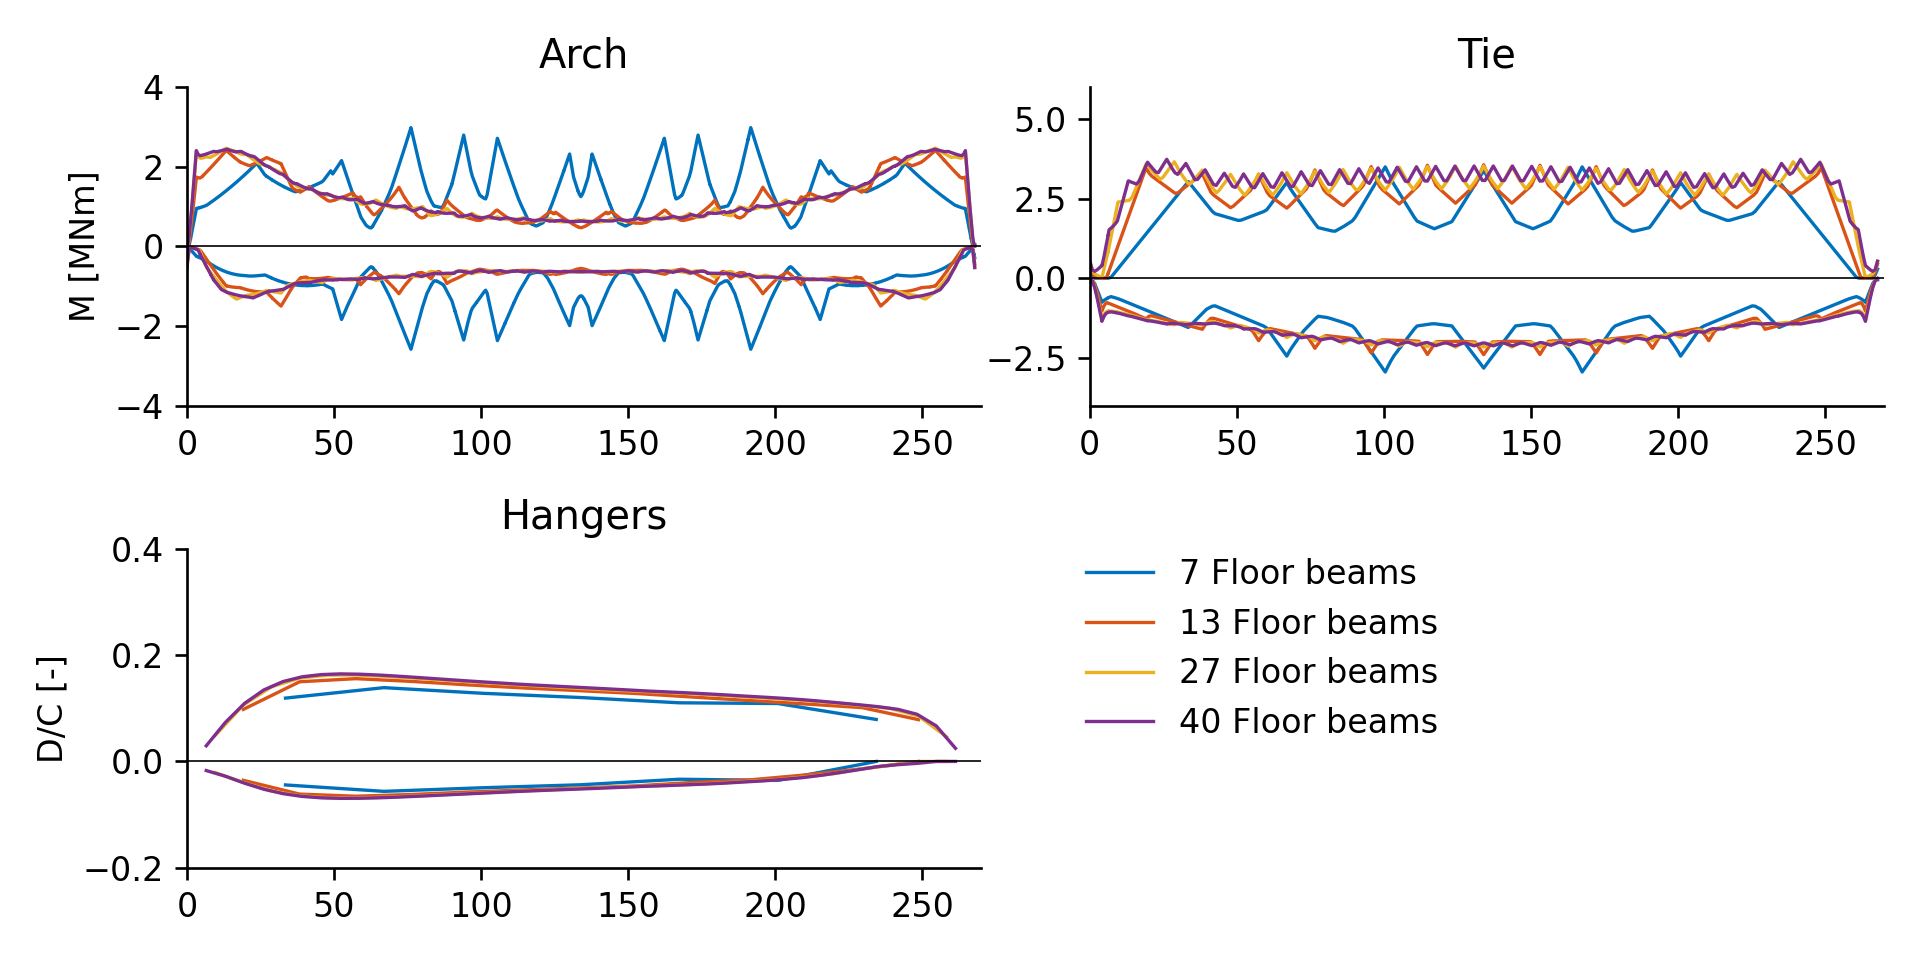
\includegraphics[trim={0 0.4cm 0 0.4cm},clip, width=0.78\textwidth]{calculations/floor beam comparison/live loading.png}
    \caption{Elastic effects under live loading for different floor beam densities}
    \label{fig:fb_live}
\end{figure}

\begin{table}[H]
    \centering
    \resizebox{\columnwidth}{!}{%
    \input{calculations/floor beam comparison/dc comparison.txt}
    }
    \caption{Design verifications for different floor beam densities}
    \label{tab:fb_dc}
\end{table}

The extreme event of cable loss is well controlled by a denser hanger arrangement, as was already observed in the previous chapter. The impacts on the other design verification are comparably small. Both the hangers and the tie girder undergo a decrease of about 0.05 in the demand over capacity ratio. The effect ranges for the strength-I limit state are shown in Fig. \ref{fig:fb_strength} for further details. Considering the arch, 10 floor beams with an optimised shape or 27 floor beams show a well balanced moment distribution. However, also the moments in the other models do not have a decisive influence on the design.

\begin{figure}[H]
    \centering
    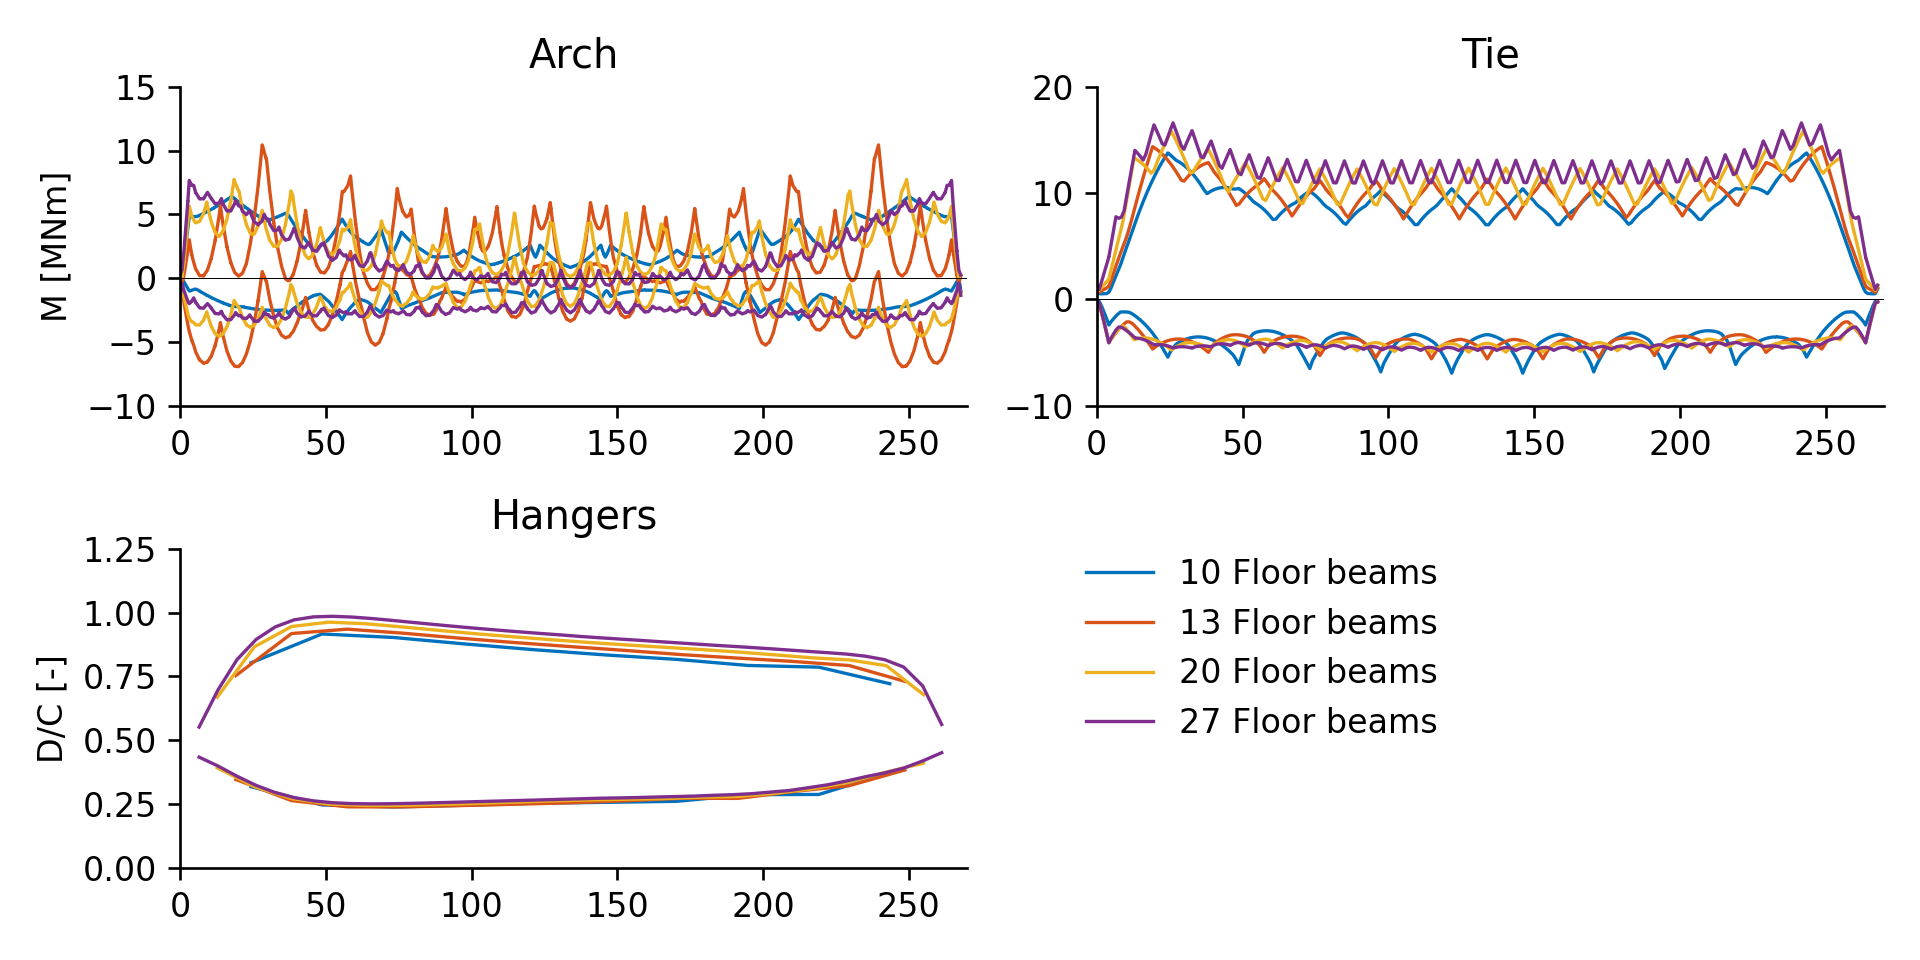
\includegraphics[trim={0 0.4cm 0 0.4cm},clip, width=0.78\textwidth]{calculations/floor beam comparison/strength-I.png}
    \caption{Strength-I effects for different floor beam densities}
    \label{fig:fb_strength}
\end{figure}

[Beschreibung des Kostenverlaufs]

\begin{figure}[H]
    \centering
    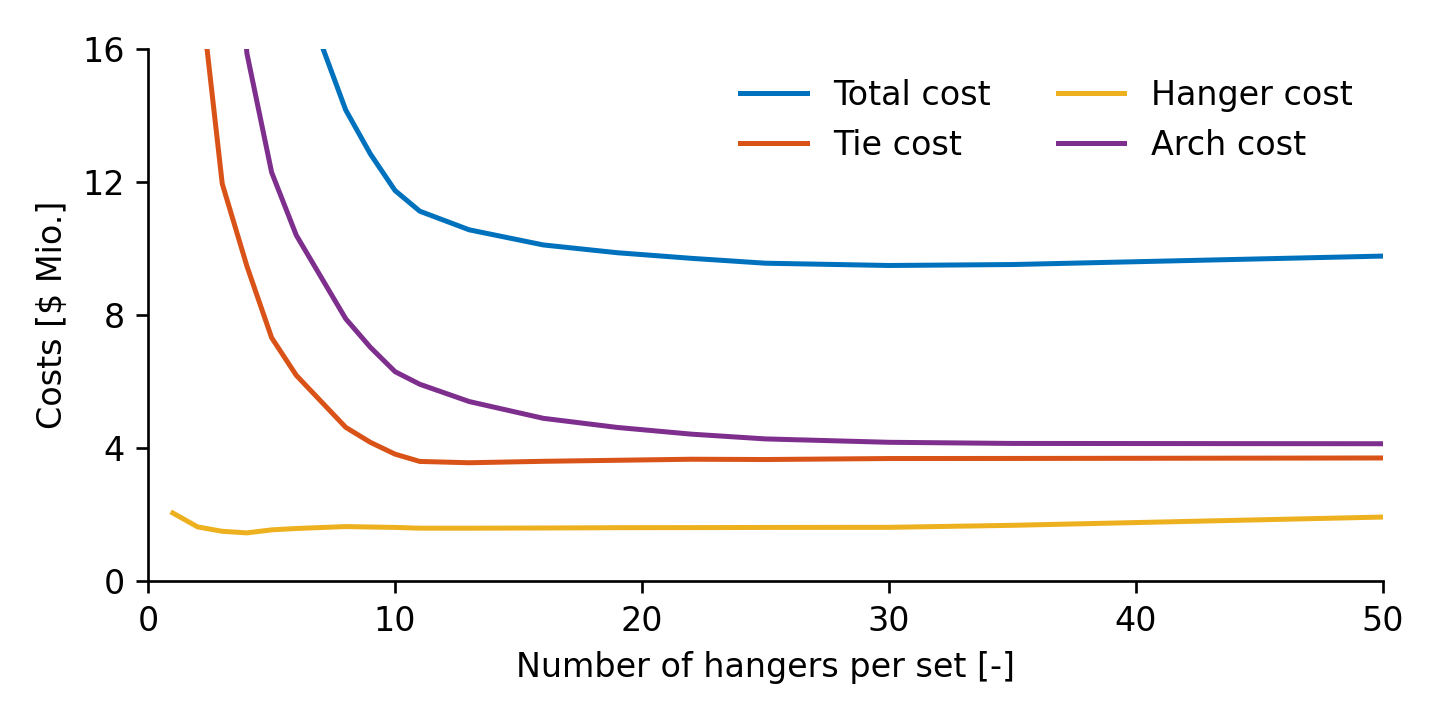
\includegraphics[width=0.7\textwidth]{calculations/floor beam comparison/cost comparison.png}
    \caption{Estimated costs for different floor beam densities}
    \label{fig:fb_costs}
\end{figure}
